\mychapter{3}{methodology}

%I plan on adding a short explanation on the importance of non-Euclidean versus Euclidean metrics. The main idea is that using  van Rossum distances implicitly assumes that the underlying neuronal response space has a vector space structure which is not always true.
%For instance, subtracting two spike trains does not make sense. Moreover, the notion of a ``basis" of the neuronal response space is undefined since it would have to depend on the number of neurons  in the space. Stay tuned for more on this......

%-----------------------------------------------------------------------------------------
%-define the two variables: firing rate and previous time
%-describe the firing rate model.
%-say that generated spikes based on that model using a non-homogeneous poisson process
%--describe the nature of the data and how previous time data is constructed.
%---describe the van rossum distance
%---describe the victor and purpura metric 
%---describe what the diffusion maps algorithm does


\section{Representation of spike trains}
Even if the size, shape and amplitude of action potentials is somewhat different,
action potentials are often viewed as identical events which occur at a single moment in time. Thus a sequence of action potentials conveys information through the precise time at which  a spike occurs. A spike train is an increasing sequence of recorded times at which a neuron fires an action potential. Spike trains are considered as the main mode of information transmission in the nervous system.  A spike train T$_{i}^{j}$ for  a single neuron labeled j is a sequence of spike times T$_{i}^{j} = \{t_{1}^{j}, ....., t_{n_{i}}^{j} \} = \{t_{i}^{j}\}$ where $0 \leq t_{1}^{j} < t_{2}^{j}< ... < t_{n_{i}}^{j} \leq T$  and  $n_{i} \geq 0$ is the number of spikes in the spike train.\\
In this case, the start and end times of a trial duration over which spikes are recorded is 0 and T respectively. Spike trains can be represented in form of Raster plots (see figure \ref{fig:Raster}).\\
 
 \begin{figure}[H]
  \centering
    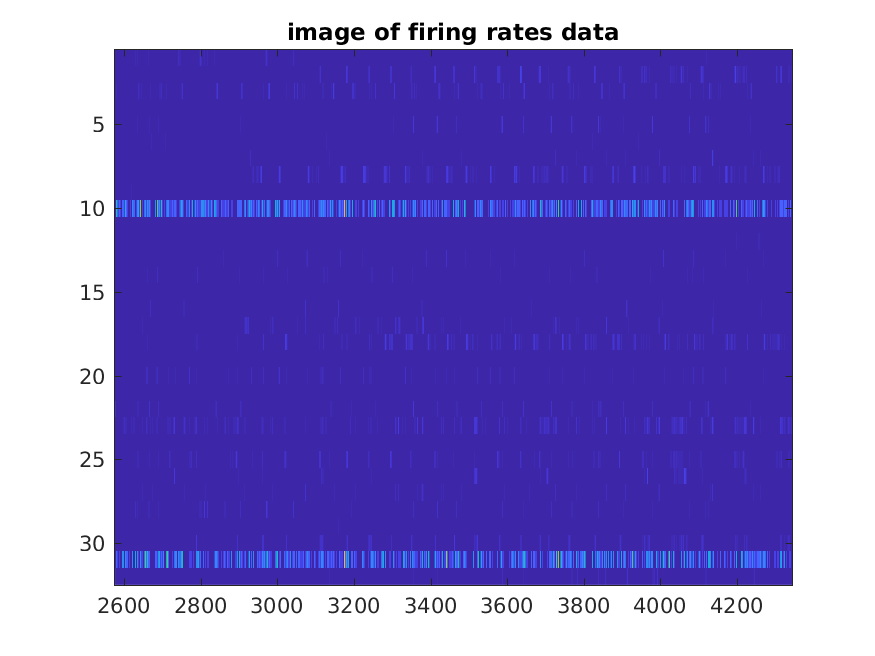
\includegraphics[scale=0.5]{Firing_Rates.png}
     \caption{A Raster Plot}
     %label the figure so latex can reference it
      \label{fig:Raster}
\end{figure}

%\footnote{An example footnote}.

\subsection{Detailed description}
A spike train can also be represented as a sum of Dirac $\delta$ functions translated
to the right by given spike times \cite{Dayan2001}.
\begin{equation}\label{spiketrain}
 T_{i}^{j}(t) =: \sum_{i=1}^{n_{i}} \delta(t-t_{i}^{j})  
\end{equation}
Equation \eqref{spiketrain} represents the spike train $T_{i}^{j}$ of the $j^{th}$ neuron consisting of $n_{i}$ spikes occurring at times $t_{i}^{j}, i = 1 \ldots n_{i}$ where $t_{i}^{j}$ denotes the $i^{th}$ spike time of the $j^{th}$ neuron.  $T_{i}^{j}$ is referred to as the response function.\\

The Dirac  function denoted $\delta(x)$ is defined by
\begin{Def}
\[
  \delta(x) =
  \begin{cases}
                                   0 & \text{if $x \neq 1$} \\
                                   \infty & \text{if $x=0$} 
  \end{cases}
\]
\end{Def}
As a "measure" on $\mathbb{R}$, we define
\begin{equation} \label{DiracDelta}
\displaystyle \int_{\mathbb{R}}  \delta(x)f(x) \quad dx = f(0) 
\end{equation}
where $f$ is any continuous function which vanishes outside a closed 
and bounded domain.\\


%use properties of a delta function to derive a definition
% for a trial average.
% also talk about a peristumulus time histogram as a way of taking into account
% temporal patterns.
%but smaller bin width implies that the resulting responses are going to be correlated
% since some spikes may belong to two different bins.
% it still does not deal with response variability 
% dimensionality reduction is a way to deal with response variability, redundancy
% correlated responses.




The  spike train \eqref{spiketrain} can also be represented as a continuous function of time by filtering (convolving) with a Kernel K as shown below:

\begin{align*}
\displaystyle
R^{j}(t) := T_{i}^{j}(t)*K(t) &= \int_{\mathbb{R}} T_{i}^{j}(t-s)K(s)  ds \\
& = \int_{\mathbb{R}}    \sum_{i=1}^{n_{i}} \delta(t - s -t_{i}^{j}) K(s)  ds 
\quad (\text{by equation \ref{spiketrain}  })  \\
& =  \int_{\mathbb{R}}    \sum_{i=1}^{n_{i}} \delta( -(s - t + t_{i}^{j})) K(s)  ds\\
& =  \sum_{i=1}^{n_{i}}   \int_{\mathbb{R}} \delta(s - (t - t_{i}^{j})) K(s)  ds \quad (\text{ since $\delta(x)$ is even and we have a finite sum})\\
& = \sum_{i=1}^{n_{i}} K(t-t^{j}_{i}) \quad (\text{by equation \ref{DiracDelta} })
\end{align*}

Thus
\begin{equation} \label{firerate}
R^{j}(t) = \sum_{i=1}^{n_{i}} K(t-t^{j}_{i})
\end{equation}


The function $R^{j}(t)$ is often referred to as the firing rate of the $j^{th}$ neuron. 
Note that $R^{j}(t)$ is independent of the precise timing of a spike.
Smoothing equation \eqref{spiketrain} with a kernel K enables us to represent events like spikes as continuous functions of time. R$^{j}$(t) is then viewed as an element of the infinite dimensional vector space of continuous functions.  Equation \eqref{firerate} 
is also referred to a filtered spike train in spike metrics literature.
The function $R^{j}(t)$ can also be viewed as an estimate of the unknown stimulus.
(cite van Rossum's paper). 
The common kernels used for estimating the firing rate include the Gaussian kernel,  decaying exponential kernel and Box car window.

% write an equation of these kernels and define what a kernel means
% copy and paste this from the kernel review you wrote on Xu's unpublished work.


\section{Description of types of metrics/distances}

Still working on this.....

% describe edit-distance, van-Rossum distance, diffussion maps description
\section{Our framework}

%------introduce our framework
%------general idea of dimensionality reduction
%-----define data transformation $X(t_n)$
%-----similarity measure $d(x_i, x_j)$
%-----algorithm (general steps)\\

A mathematical model based on the point-process framework is the best approach for 
modeling  data from the CA1 region of the rat hippocampus for two reasons.
First, the position of the animal is coded by place cells using both the firing rate
and the precise time at which the cells fire with respect to the hippocampal theta rhythm.
The theta rhythm is a sinusoid of frequency 7-12 Hz which occurs whenever a rat changes
position in  a specific direction \cite{OKeefe1971, Burgess1993}.
Second,  metrics based on the point-process viewpoint are often non-Euclidean \cite{Aronov2004, Victor2005}. Moreover, there are specific examples like sensory space in  the olfactory system and the perceptual space of color vision which are typically non-Euclidean and analysis in the point-process framework would be most appropriate.\\


\subsection{Our approach}

We propose a method of pre-procesing spike times by looking at the time since the 
last spike (previous time), smoothing the previous time using the Laplace kernel
and then using the diffusion distance \cite{coifman2006diffusion} as a measure of similarity
between spike trains. The low dimensional model is obtained by non-linear dimensionality reduction using the diffusion maps algorithm. The measure of ``goodness" of our low dimensional model is done by comparing the mutual information  \cite{quiroga2009extracting, Dayan2001}  between the resultant eigen vectors and and the position of the animal. We test our results using both simulations and behavioral real-world data.\\


























%\begin{itemize}

%========suggested by Duane=========================================
%\item  First mention that there is a general conceptual framework
%namely dimensionality reduction and then say that
% the metric a approach is just one of the ways of doing dim reduction
% yet ensuring minimal information loss.

%\item The previous/next time approach is our new way of preprocessing
% the data and then using some of the usual metrics to analyze it.

%============end suggestion=========================================
%\item How did you create the metric and what precisely is it's definition?
%\item Experimental design. Discuss how the data was collected using a diagram
%\item Mention that this kind of analysis has never been 
%applied to this Redish Lab data.
%\item describe your methodology starting with the fake brain model and then tests on real data
%\item what are the names and definitions of the algorithms you're using?
%\item what is dimensionality reductions and why are you using linear instead of non linear
%\item Why did you choose this particular algorithm(s)?
%\item What is wrong with using PCA or Kernel PCA?
%
%\end{itemize}





